\section{Introduction}
In this chapter will be presented the architecture of CPIM especially for the NoSQL service as it was before this work, then will be explained how was possible to include Kundera as persistence layer for the NoSQL service in CPIM and what problem has been faced during the process.
Furthermore in section \ref{sec:hegira} is shown how the integration with the migration system \textit{Hegira} has been introduced, what are the feature supported by this integration and which design choices has been put in place. 

\section{CPIM architecture}
To be able to expose a common interface for the multiple services supported by the library, CPIM adopts heavily the factory and singleton patterns.

\noindent The main access point of the library is the \texttt{MF} (Manager Factory) a singleton object which is responsible of reading the configuration files and exposing a set of methods that will build instances for the service factories.
The initialization is done through the first call to \texttt{MF.getFactory()} which read the configuration files and build an instance of \texttt{CloudMetadata} which will be referenced by all the other services and contains all the information stored in the configuration files.
 
\newparagraph The library is organized in several packages each of one is responsible of a particular service.
\noindent Each service exposes a factory class which is invoked through the \texttt{MF} factory, the service factory maintains a singleton instance of the provider-specific service implementation which is built at the first call based on the configuration available inside the singleton instance of \texttt{CloudMetadata}.
The result of this process is that with the same method call, based on the configuration file, is instantiated one service implementation or another.

\subsection{NoSQL service}
Before this work CPIM library supports NoSQL interaction through Java Persistence API.
The interoperability with the supported clouds is made possible thanks to the previously described factory pattern, a complete class diagram for this service can be seen in the figure \ref{fig:cpim-nosql}.

\begin{figure}[tbh]
  \centering
  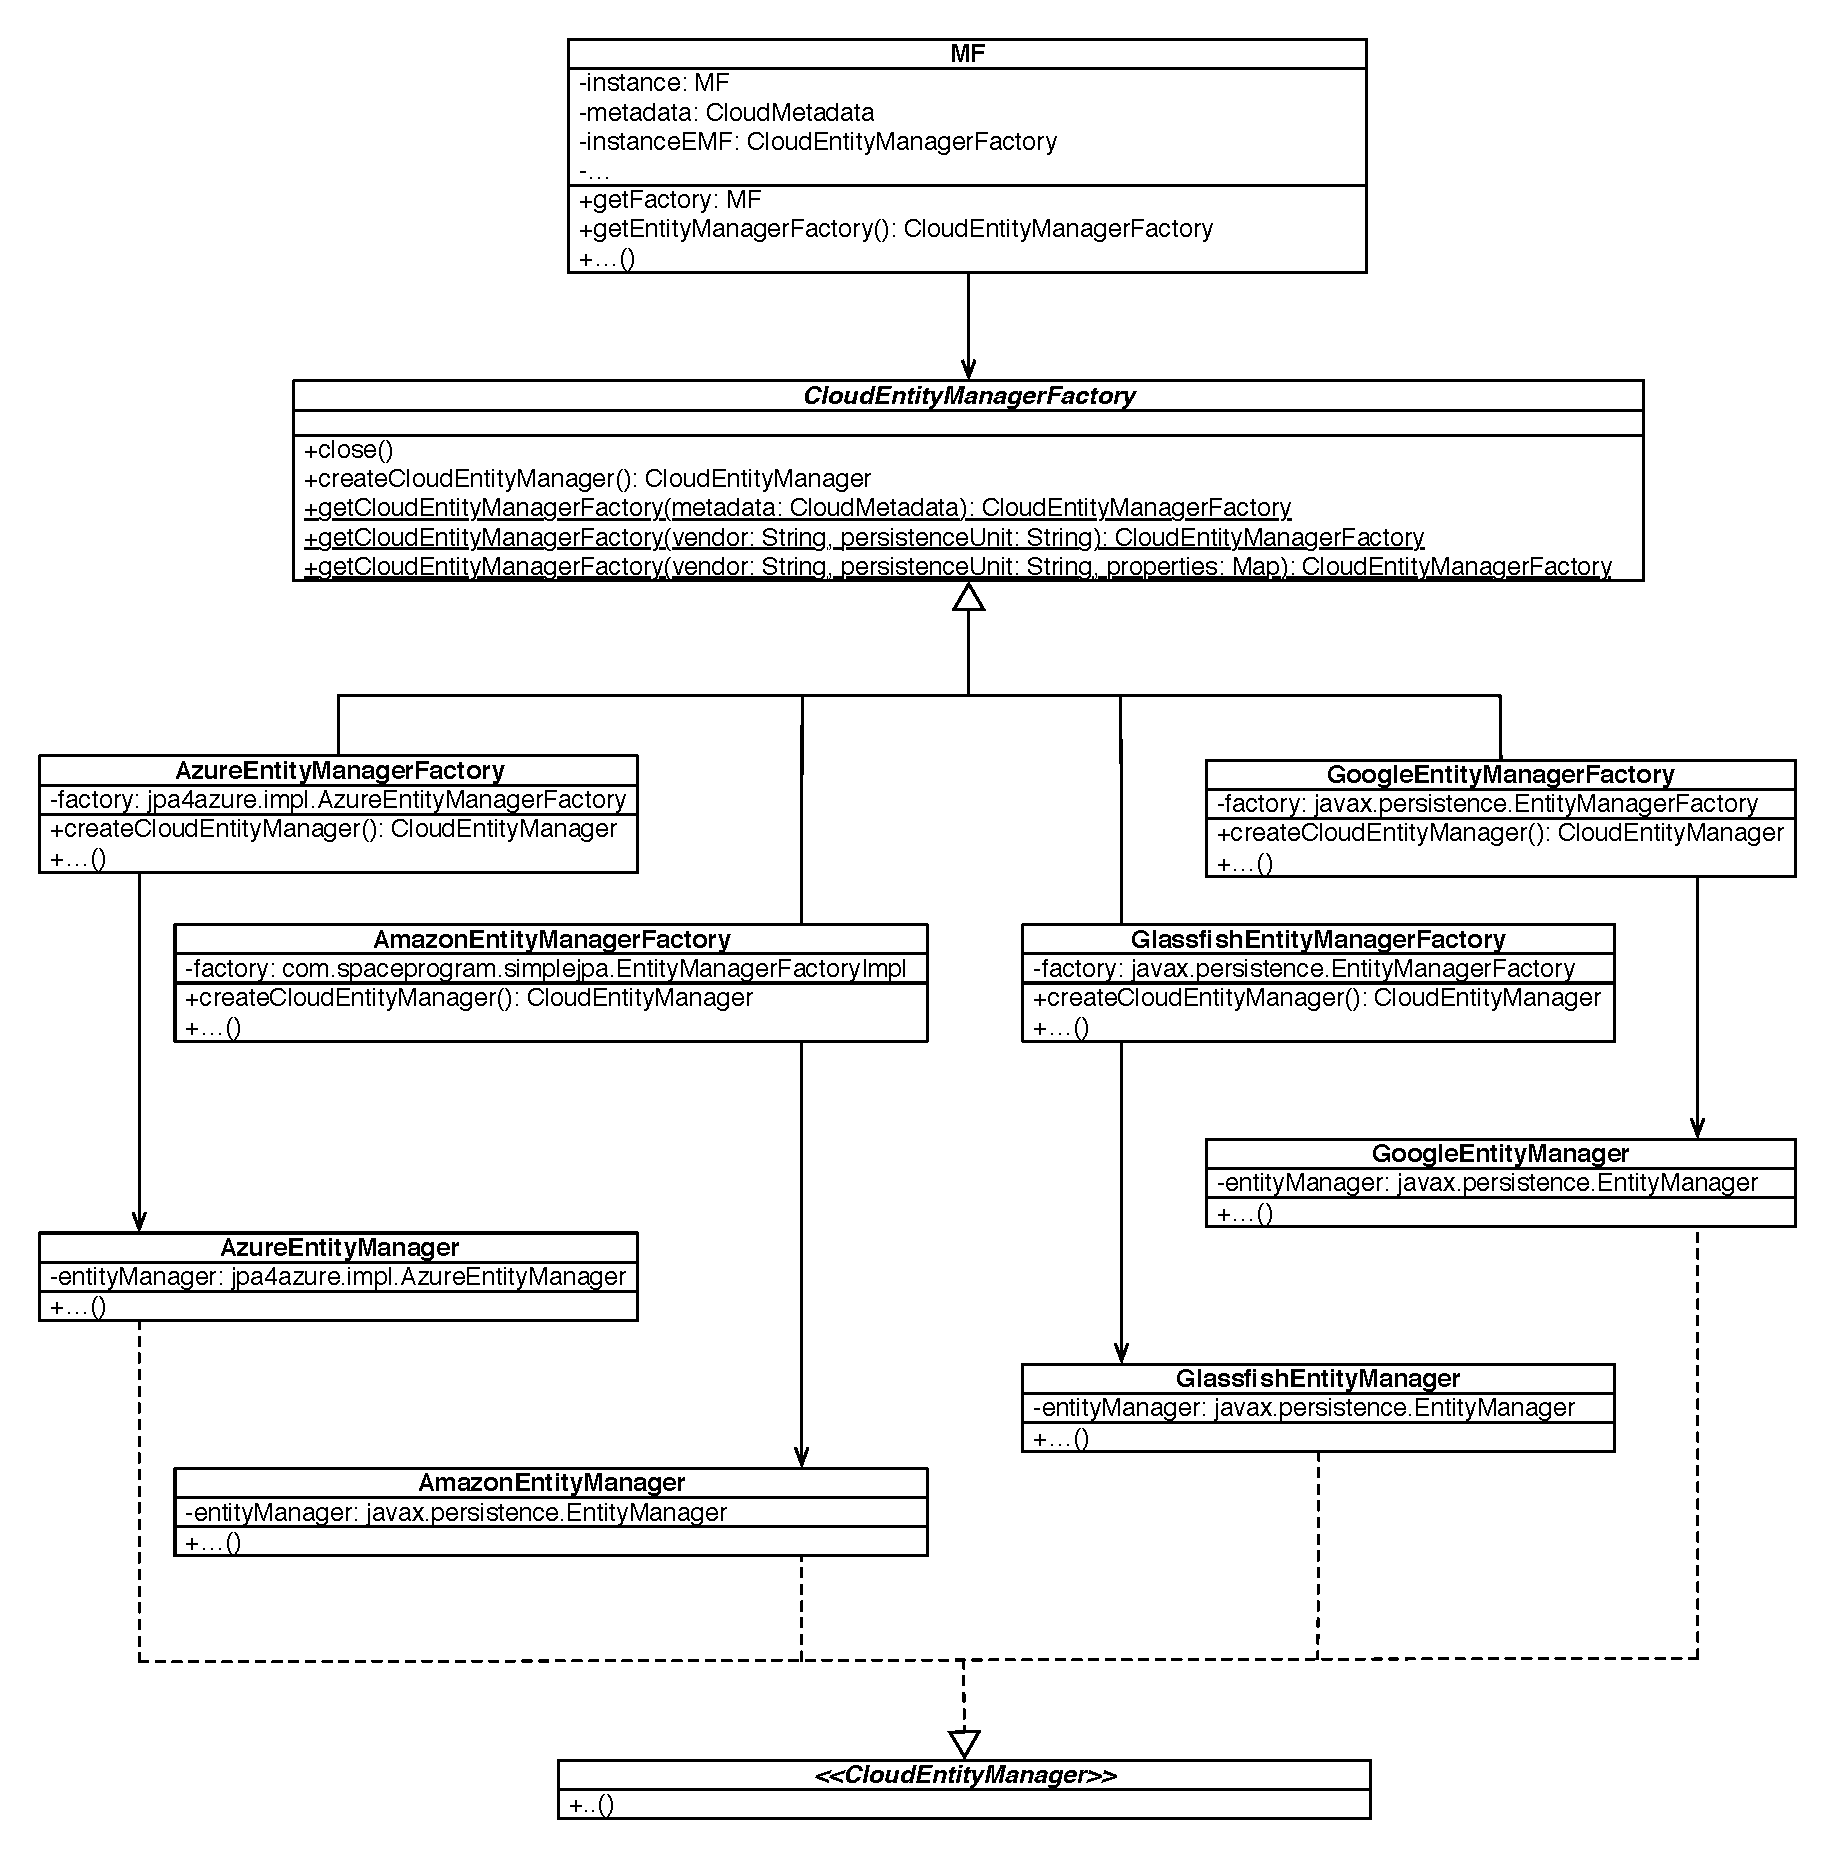
\includegraphics[width=14cm]{images/cpim_nosql_old}
  \caption{NoSQL service architecture}
  \label{fig:cpim-nosql}
\end{figure}

\noindent To use the service, the first step is instantiate a \texttt{CloudEntityManagerFactory} and, depending on the configuration file, this factory instantiate the vendor specific factory. For example in case that Google is the chosen vendor, the instantiated factory will be \texttt{GoogleEntityManagerFactory}. 
Each provider-specific \texttt{EntityManagerFactory} is responsible of instantiating an \texttt{EntityManager} which is the gateway to the underlying database. All the vendor-specific \texttt{EntityManager}(s) implement the common \texttt{CloudEntityManager} interface to achieve uniformity in methods and behavior.
The various implementation of the \texttt{CloudEntityManager} delegates every method call to the vendor-specific persistence provider. 

\newparagraph JPA is not a default language for NoSQL (as described in chapter \ref{chapter:sota}) but, due to its wide usage among Java developers, several JPA implementation has been build upon various NoSQL databases both developed by the vendor of the NoSQL storage or by the community.
This means that to support the NoSQL service through the JPA interface, an implementation of the JPA interface must be found. There are so three different persistence providers, one for each cloud provider:
\begin{itemize}
\item for \textit{Google Datastore} its used an official JPA implementation, available inside the SDK
\item for \textit{Amazon SimpleDB} its used \textbf{SimpleJPA}, a third-party implementation of the JPA interface
\item for \textit{Azure Tables} its used \textbf{jpa4azure}, a third-party implementation of the JPA interface
\end{itemize}

\noindent There are couple of things to notice: Amazon SimpleDB has been deprecated in favor of DynamoDB and \textit{jpa4azure} is not being maintained anymore, therefore CPIM needs to be updated in order to get rid of those outdated software.

\section{Kundera integration}
To solve this problems and reduce the number of software on which the CPIM rely on to provide the NoSQL service, the proposed solution  to modify the current CPIM architecture with a unique persistence provider that has been identified in Kundera.

\newparagraph The proposed solution is resumed in the architecture of figure \ref{fig:cpim-kundera} in which the benefit of having a single JPA provider are clearly visible. The architecture is slightly less articulated and no check on the selected provider is needed since this is handled by Kundera while reading the \texttt{persistence.xml} file in which the user will define what datastore is interested in.
Another benefit of this architecture is that the choice of the NoSQL technology is no more bound to the vendor specified in the CPIM configuration file, is in fact possible deploy the application in one of the supported PaaS provider and choose as NoSQL solution of another one which will be addressed remotely, simply by configuring the \texttt{persistence.xml}, moreover it's possible exploiting the Kundera polyglot persistency, to persist part of the data in a database and another part in another one defining the persistence units properly.

\begin{figure}[tbh]
  \centering
  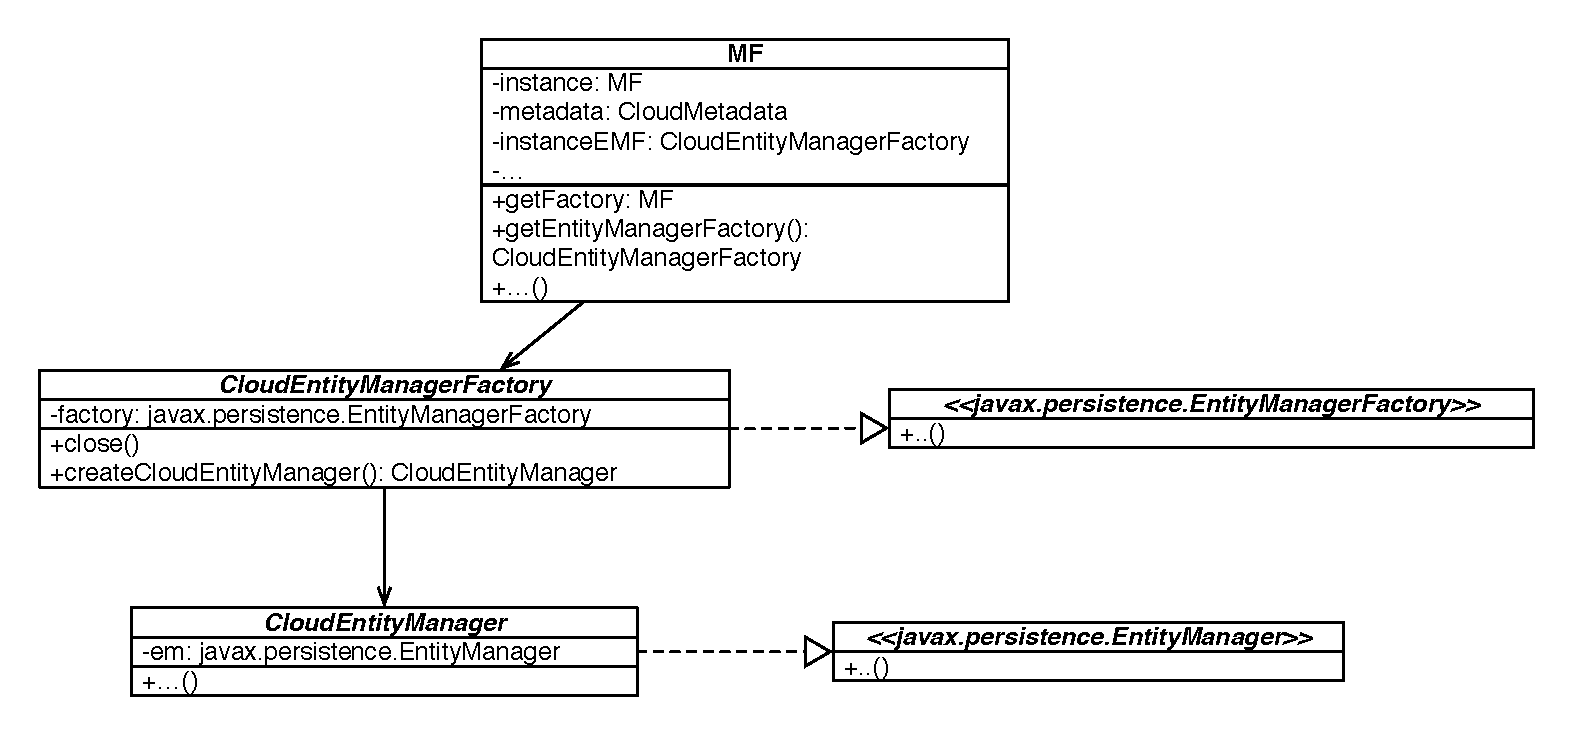
\includegraphics[width=14cm]{images/cpim_nosql_kundera}
  \caption{The modified NoSQL service architecture TODO add interfaces}
  \label{fig:cpim-kundera}
\end{figure}

\noindent The actual implementation is completely provider agnostic in the sense that actually Kundera is not required as depencency and in fact is not listed as a dependency for CPIM. At runtime, when a Kundera client will be listed in the dependency of the user application, as well as CPIM, the persistence provider dependency will be satisfied.
This is due to the fact that the \texttt{CloudEntityManagerFactory} and the \texttt{CloudEntityManager} implements respectively the JPA interfaces  \texttt{EntityManagerFactory}  and \texttt{EntityManager}.
The actual call to the runtime provider is within the \texttt{CloudEntityManager} that on construction instantiate an instance of the provider \texttt{EntityManager} and uses that reference to delegate every method execution to it.

\noindent This can seems a over-designed architecture but it tourns out to be extremely necessary in order to provides a transparent interaction with the migration system as it will explained later on in this chapter.

\subsection{Problems encountered}
Kundera provides an uniform access through the JPA interface independently from the provider, which is somehow defined in the \textit{persistence.xml} through the Kundera client selection. For this reasons all the old libraries that provides a JPA implementation for a specific provider can be removed from the CPIM. 
This tentative in cleaning the dependency of CPIM caused two main problems:
\begin{enumerate}
\item \textit{jpa4azure} turns out to be used also for Queue and Blob service of Windows Azure
\item Kundera seems to have problem when multiple persistence provider are found in the classpath and has not be found a way to force the selection of Kundera as persistence provider (besides specifying it in the \textit{persistence.xml} file)
\end{enumerate} 

\noindent To solve the first problem, the code of the extended version of\textit{jpa4azure} has been inspected since it was extended to support some missing functionalities of the JPA interface, the library contains two main packages:
\begin{itemize}
\item \texttt{jpa4azure}, which contains the code that implement the JPA
\item \texttt{com.windowsazure.samples}, which contains the code do ease the communication with the Azure services
\end{itemize}
The \texttt{jpa4azure} package has been removed and the library rebuild since the other package is the one used in the Blob and Queue service. Its possible to completely remove \texttt{jpa4azure} but is necessary to rewrite also the CPIM Blob storage service for Azure using the Azure SDK.

\newparagraph CPIM shows more errors in the code in the Queue service and after some investigations, turns out that when \textit{jpa4azure} was extended the class \texttt{AzureQueueManagerFactory} and other were introduced.
The problem was that \texttt{AzureQueueManagerFactory} use the JPA interface to communicate with the Queue service so removing the support to JPA interface has leaded to lose the support to Azure Queue service.
One possible solution to this would be rewrite the CPIM Queue services for Azure using Azure SDK.

\section{Hegira integration}
\label{sec:hegira}
To support data synchronization and migration, the NoSQL service was further modified to integrate with \textbf{Hegira} \cite{thesis:marco}. An high level schema of the interaction we want to achieve is reported in figure \ref{fig:high-level-interaction}

\begin{figure}[tbh]
  \centering
  %\includegraphics[width=14cm]{}
  \begin{minipage}[c][0.33\textheight][c]{0.5\textwidth}
  \end{minipage}
  \caption{High level schema of interaction TODO}
  \label{fig:high-level-interaction}
\end{figure} 

\noindent As can be stated from the schema, the CPIM library needs to connect to the migration system on order to understand when migration is in progress and in that case only bypass the interaction with Kundera by building a string representation of the user operation in a SQL format, then this string is sent to the commit log of \textit{Hegira} that then will pop the statements and translate the SQL statement into a datastore-specific operation.

\subsection{Migration Manager}
Interaction with the migration system is handled primarily by the \texttt{MigrationManager} class which follows a state pattern represented in the class diagram \ref{fig:migration-class-diagram}. 
 
\begin{figure}[tbh]
  \centering
  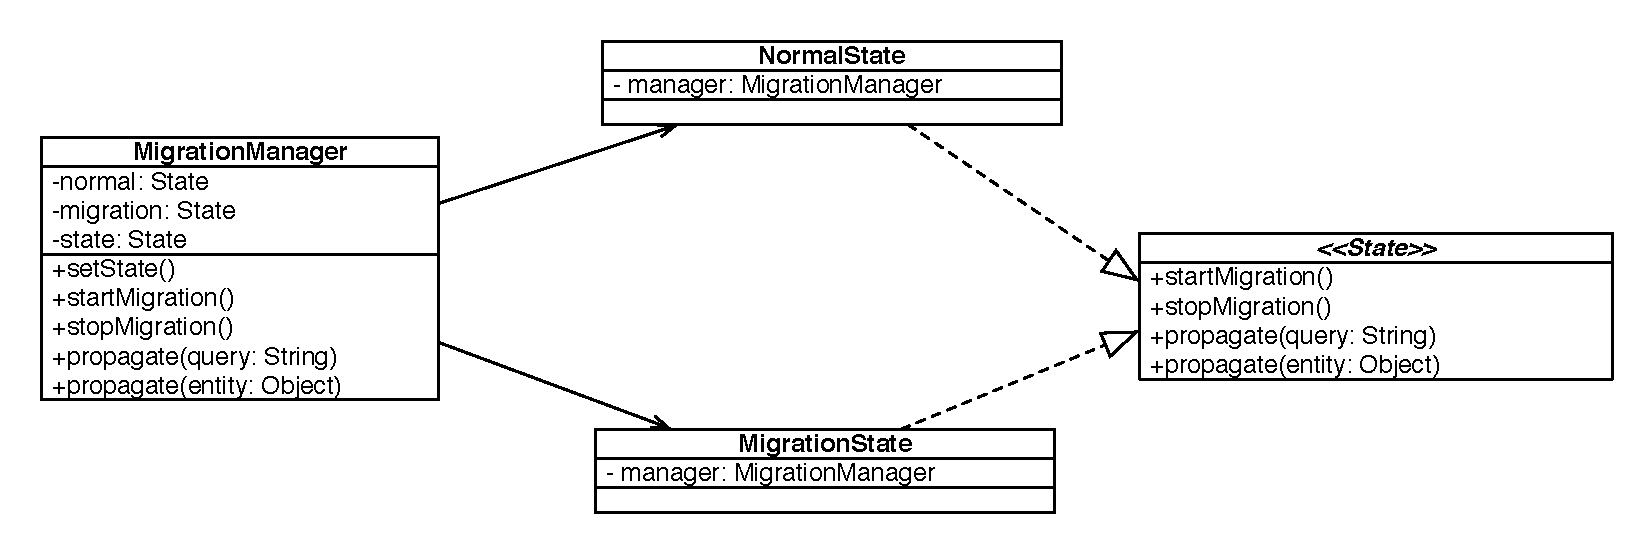
\includegraphics[width=14cm]{images/migration_class_diagram}
  \caption{\texttt{MigrationManager} class diagram}
  \label{fig:migration-class-diagram}
\end{figure} 

\noindent The pattern permits to the \texttt{MigrationManager} to delegates the method execution to the current state, the state diagram is the one represented in figure \ref{fig:migration-fsa} is and composed by two states \texttt{Migration} and \texttt{Normal} that encapsulate the required behavior.
    
\begin{figure}[tbh]
  \centering
  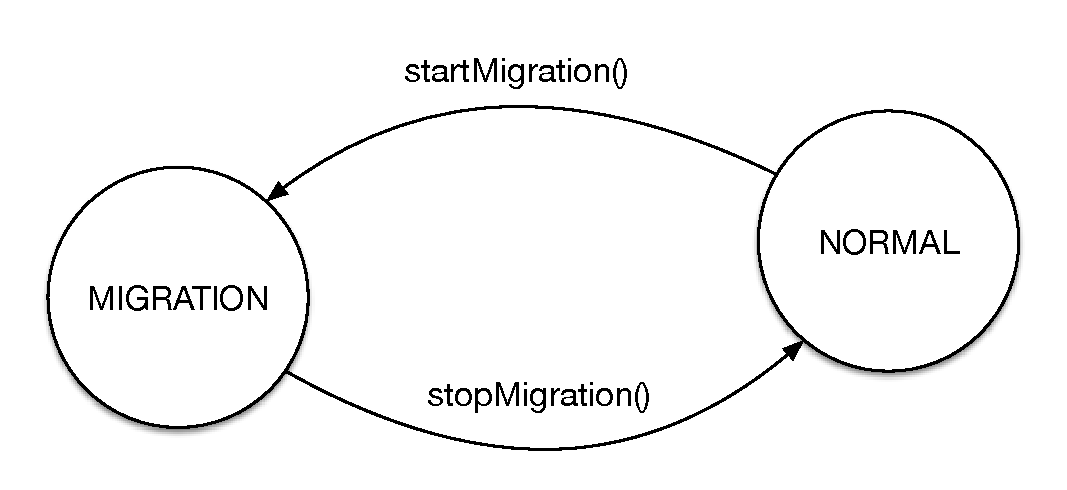
\includegraphics[width=6cm]{images/migration_fsa}
  \caption{\texttt{MigrationManager} states}
  \label{fig:migration-fsa}
\end{figure} 

\noindent This part of the design was actually made before knowing exactly how the interactions will exactly be since the component to interact with were not finished yet. Hence in order to have a well-defined place in which behavior has to be encapsulated, the state pattern was the best solution even for future extensibility in case the interaction with the migration system will become more complex.  

\section{Intercept user operations}
The first operation that needs to be analyzed is where is possible to intercept user operation is a way that is completely transparent to the user.
The operation that we want to intercept are the insert, update and delete operation cause those are the operation that alter the structure of the data and thus are the one that needs to be processed by the migration system.

\subsection{Intercepting CRUD operations}
CRUD operation are always handled in the \texttt{EntityManager}, three are the methods that needs to be intercepted:
\begin{itemize}
\item \texttt{EntityManager.persist(Object entity)} for the insert operation
\item \texttt{EntityManager.merge(Object entity)} for the update operation
\item \texttt{EntityManager.remove(Object entity)} for the delete operation
\end{itemize}
\noindent User is not directly invoking method on the provider entity manager but interacts with the persistence provider through the \texttt{CloudEntityManager} class. Without the support for the migration system the \texttt{CloudEntityManager}, as stated previously, delegates every method call to the provider entity manager.
To integrate migration and synchronization logic, the methods mentioned above should contain a little more amount of logic shown in the snippet of code \ref{code:isMigrating} taking as example the update operation.

\begin{algorithm}[h]
  \begin{algorithmic}[1]
    \Procedure{EntityManager.merge}{$object$}   
      \If{MigrationManager.isMigrating()}
        \State MigrationManager.propagate($object$, OperationType.UPDATE)
      \Else
        \State // delegate operation to the provider
      \EndIf
    \EndProcedure
  \end{algorithmic}	
  \caption{Integrate migration logic}
  \label{code:isMigrating}
\end{algorithm}

\noindent In case of migration is visible the call to the \texttt{propagate} method. It accept two arguments:
\begin{itemize}
\item the entity to be converted to a statement
\item the operation that needs to be generated
\end{itemize}
The method is called on the \texttt{EntityManager} which then delegates the execution to the current state which should be the migration state at that point. The \texttt{propagate} method of the migration state is responsible of building the requested statements using the statement builders and then sending the generated statements to the commit log of \textit{Hegira}. Both action are described in detail later on.

\subsection{Intercepting queries}
A first look at the JPQL specification \cite{book:projpa2} revealed that JPQL does not support \textit{INSERT} statements and so the only way user have to persist entities is through \texttt{EntityManager.persist(Object entity)} that is one of the case described in the previous section, so only the remaining cases (\textit{UPDATE} and \textit{DELETE}) needs to be intercepted.

\noindent JPA interface provides several ways to build and execute queries all available by calling the proper methods defined in the \texttt{EntityManager} interface: 
\begin{itemize}
\item \texttt{createQuery} from JPQL query string
\item \texttt{createQuery} from an instance of \texttt{CriteriaQuery}
\item \texttt{createNamedQuery}
\item \texttt{createNativeQuery}
\end{itemize}
 
\noindent Native queries are clearly not supported by Kundera and thus from the migration system clearly because there not so many storage that provides a SQL-like language to specify queries.
Create queries through \texttt{CriteriaQuery} is currently not supported.
The remaining two kind of methods to create queries are slightly different to handle.

\subsubsection{Queries through EntityManager}
TODO

\subsubsection{Named Queries}
TODO

\noindent Named queries metadata are maintained inside the \texttt{PersistenceMetadata} class. This class, besides maintaining information about named queries, maintains principally a mapping between table names and their class canonical name (full package plus the class name). The content of this class is built the first time is queried (since is a singleton instance) and does not read directly the  configuration files but reads the \texttt{CloudMetadata} instance that has been modified to include all the required parameters that needs to be read from configuration files. 
Information of table to class mapping is required for statements building and for sequence number handling both described later on.
 
\section{Synchronization}
\label{sec:synch}
In the previous section, an overview of the required logic that has been built to integrate \textit{Hegira} was described. Now let's face the problem of synchronization that allows the migration to be performed live.

\noindent A special look needs to be reserved for the insert operation. When the user updates or delete an entity no matter if through the entity manager or through a query, he already knows the identifier of that entity since the insert operation have already persisted the entity into the underlying database and thus generated the identifier.
Since we want to guarantee a synchronization with the migration system, user cannot define its own identifiers but them needs to be assigned from the migration system.
The main caveats is that such assignment has to be made even if the migration is not running yet so the identifier assignment has to be made in two cases:
\begin{enumerate}
\item insert statements built from persist operation during a migration phase
\item \textit{standard} insert operation through the entity manager during a normal state
\end{enumerate}

\noindent The solution is actually quite simple since everything can be checked inside the \texttt{EntityManager.persist} method as described in the snippet of code \ref{code:persist}.

\begin{algorithm}[h]
  \begin{algorithmic}[1]
    \Procedure{EntityManager.persist}{$object$}   
      \If{MigrationManager.isMigrating()}
                \State MigrationManager.propagate($object$, OperationType.INSERT)
      \Else
        \State $id \gets$ SeqNumberProvider.getNextSequenceNumber($table$)
        \State $object$.setId($id$)
        \State // delegate operation to the provider
      \EndIf
    \EndProcedure
  \end{algorithmic}	
  \caption{Persist operation}
  \label{code:isMigrating}
\end{algorithm}

\noindent In the code snippet is visible a call to the  \texttt{SeqNumberProvider} class which is the class responsible of actually interacts with the synchronization service of Hegira and handle the \textit{sequence numbers} i.e. the entities identifiers defined by Hegira to achieve synchronization. 

\newparagraph TODO flow chart ??

\subsubsection{Handling the sequence numbers}
The sequence numbers are handled by the class texttt{SeqNumberProvider}, a singleton instance that provides a simple way to get the assigned sequence numbers per table.
\noindent The class diagram of this component and of the component it interacts with is shown in figure \ref{fig:seq-provider}

\begin{figure}[tbh]
  \centering
  %\includegraphics[width=14cm]{}
  \begin{minipage}[c][0.33\textheight][c]{0.5\textwidth}
  \end{minipage}
  \caption{Sequence numbers handling architecture TODO}
  \label{fig:seq-provider}
\end{figure} 

\noindent The \texttt{SeqNumberProvider} keeps an instance of \texttt{SeqNumberDispenserImpl} for each table that needs to be persisted. The \texttt{SeqNumberDispenserImpl} is responsible of managing and maintaining the sequence numbers for a specific table by requesting when necessary more sequence number to the synchronization system.
\texttt{SeqNumberDispenserImpl} is an implementation of the general interface \texttt{SeqNumberDispenser} made to be able, maybe in the future, to create more dispenser with different logics.

More in detail the \texttt{SeqNumberProvider} is responsible of:
\begin{enumerate}
\item provide a unique access point where requesting the next assigned sequence number for a table
\item initialize or restore the state of the dispenser for each of the persisted tables
\end{enumerate}
\noindent The first is performed through the method \texttt{getNextSequenceNumber(String tableName)} that delegates the operation to the correct \texttt{SeqNumberDispenser} associated to the requested table.
The second functionality is achieved by requesting to the \texttt{SeqNumberDispenser}(s) their state representation and then saving it to a Blob storage or to file depending to the configuration file \textit{migration.xml} described in appendix \ref{app:migration}. The restoring phase is performed on construction, if a backup exists, either on file or on the Blob storage, the \texttt{SeqNumberDispenser}(s) are initialized giving them their state representation to restore.
This mechanism in which the \texttt{SeqNumberProvider} is completely agnostic to the actual state representation of the \texttt{SeqNumberDispenser}(s) make future extensibility more easy and less constrained.

\noindent The list of all the tables to be persisted is retrieved from the \texttt{PersistenceMetadata} mentioned previously for named queries.
 
\subsection{Contacting the synchronization system}
The interaction with the synchronization system as now was only described as a method call. Those calls are made on an external library (\texttt{zkWrapper}) that connects to a zookeeper instance to communicate with the synchronization system and receive the assigned sequence numbers.
Since the zookeeper library issues threads to handle communication, was not possible to use this method for Google App Engine since the App Engine runtime does not permit to spawn thread.
Two are the feature that requires to communicate with the synchronization system and so use the \texttt{zkWrapper}:
\begin{itemize}
\item the migration state listener that modify the \texttt{MigrationManager} state accordingly
\item the \texttt{SeqNumberDispenser}(s) that needs to retrieve the sequence number assigned to tables
\end{itemize} 
\noindent The solution adopted was to modify the \texttt{zkWrapper} library to include an API version that handle the calls not by connecting directly to a zookeeper instance but contacting a remote server through some defined API that ultimately interacts with the migration system.

\newparagraph A simple structure has been built to make both the \texttt{MigrationManager} and the \texttt{SeqNumberDispenser}(s) transparent to the type of client that is used to retrieve information from the synchronization system. The architecture is shown in figure \ref{fig:zk-adapter}

\begin{figure}[tbh]
  \centering
  %\includegraphics[width=14cm]{}
  \begin{minipage}[c][0.33\textheight][c]{0.5\textwidth}
  \end{minipage}
  \caption{Interaction with the synchronization system TODO}
  \label{fig:zk-adapter}
\end{figure} 

\noindent The \texttt{HegiraConnector} is the class responsible of deciding which kind of client needs to be instantiated reading the configuration parsed  in \texttt{CloudMetadata}, the \texttt{HegiraConnector}  keeps internally an instance of the instantiated client and provides access to its method by delegation.
The two available clients implements the interface \texttt{ZKAdapter}, built to uniform the methods of the two implementations.

\paragraph{Thread-based client} If the user deploy the application on a thread-capable client and configure the \textit{migration.xml} accordingly, an instance of \texttt{ZKThread} is built. This version of the client uses directly the implementation of the library \texttt{zkWrapper} since there should not be any problem in thread spawning.
The \texttt{isSynchronizing()} methods returns a value which is keept inside the \texttt{ZKThread} instance and is queried by the \texttt{MigrationManager}.
Both the state of the \texttt{MigrationManager} and the value inside \texttt{ZKThread} are modified by the \texttt{SynchronizationListener} which is asynchronously notified by the \texttt{zkWrapper} library when the migration state change.

\paragraph{HTTP-based client} In case that threads are not supported by the cloud provider the client version that is instantiated (by looking at the configuration) is \texttt{ZKHttp} which uses the API-caller added to the \texttt{zkWrapper} library.
Since no listener can be register and asynchronously notified of a change in the migration state and is not possible to somehow cache the state or make assumption on it, each call of the \texttt{MigrationManager} to the method \texttt{isSynchronizing()} will perform an API call to the remote server and will return the state of the synchronization just queried.

\section{Build statements from user operations}
\label{sec:statements}
\subsection{Build statements from objects}
TODO
\subsection{Build statements from JPQL queries}
TODO
\subsection{Sending statements to Hegira}
TODO

\section{Interoperability of stored data}
The Kundera client developed and described in chapter \ref{chap:kundera} was developed to be as much as consistent to the other client developed for Kundera to be more likely accepted by the community and so are not built to be completely interoperable.
In an optic of data migration what we want to achieve is that data stored within a database and migrated to another one are still readable to the application without changes besides the new database configuration. 

\noindent The problem for Kundera clients are the relationships. Each database have its own ways to define identifier for the persisted entities, for Google Datastore there's the \texttt{Key} with \textit{Kind} and an \textit{identifier}, for Azure there are the \textit{partition-key} and the \textit{row-key}.Concepts are different but actually quite similar since both databases are key-value columnar database. 
A solution to the problem would have been to modify the migration system in order to make it aware of the problem and let it translate the relational columns in the format of the target database, in this way the relational columns should have been identified in some way to let the system handle them. This can be done by adding a pre-defined prefix or a suffix to those columns.
Since this solution require a good amount of changes in the migration system, other solution have been explored.
 
\newparagraph Back to the concept of identifier, generally, in columnar databases, columns are grouped in a \textit{column family} and set of columns are identified by a \textit{key}, actually the \textit{key} can span among different \textit{column families} but that's not possible either in Datastore or Azure Table.
The pair (\textit{column family}, \textit{key}) is sufficient to identify an entity (composed by one or more columns) is so needed a mapping between database-specific terminology to the more general one, this mapping is shown in table \ref{table:mapping}.

\begin{table}[h]
\begin{center}
\renewcommand{\arraystretch}{1.4}
\begin{tabular}{lcc}
\hline
\textbf{General concept} & \textbf{Datastore} & \textbf{Azure Table}\\ 
\hline\hline
Column Family & Kind & partition-key \\
Key & key-identifier & row-key \\
\hline
\end{tabular}
\end{center}
\caption{Column family and Key mapping among supported databases.}
\label{table:mapping}
\end{table}

\noindent At this point is needed a common way of save relationships as column family and key in a way that is interoperable among both the client extension.
The proposed solution is to persist \texttt{columnFamily\textunderscore key} an idea that came from the Azure Table extension which already save relationships similar to this. This solution has to be preferred w.r.t the one that require modification of the migration system since the interoperability is achieved transparently to it.

\subsection{Kundera clients modification}
Since lot of work has already been done on the Kundera clients, the modification to them has been made on a separate branch of the projects named \textit{migration}.

\paragraph{Google Datastore} The Datastore extension has been modified to persist relationships as \texttt{kind\textunderscore key-identifier} instead of the \texttt{Key} instance.
Join tables require particular care. Kundera is not providing the class of the entities involved in the join table but just the column names and the identifier (the one with the \texttt{@Id} annotation). Queries are possible even if the \textit{Kind} is unknown since Kundera provides the entity class with the entity identifier in the find operation.
To be more consistent and apply the identifier pattern (\texttt{kind\textunderscore key-identifier}) even for join tables, a map is maintained in the client and built inspecting Kundera metadata to keep track of which entity classes are involved in which many to many relationship.

\paragraph{Azure Table} The Azure Table extension has been modified too to reflect the newly defined standard for relationships. The actual problem here is that user can manually handle the partition-key but is not a possibility that can be guaranteed since if an entity is persisted with a partition-key, it will be read by the Datastore extension as of that \textit{Kind}.
Since the \texttt{Kind} in Datastore extension is the entity table name, has been decided to lock the Azure Table partition-key to the table name so user cannot decide its own since this will break the interoperability of data.
The thing to notice is that the decided pattern \texttt{partition-key\textunderscore row-key} has not been broken, the only limitation is the one that fix the partition-key to the table name.

\noindent The same discussion for the join tables made previously for Datastore applies as is also for the Azure Table extension.

\section{Summary}
In this chapter has been rapidly described the CPIM structure and the architecture of the NoSQL service before this work. Then has been described how was possible to integrate Kundera as unique persistence provider in the NoSQL service and the problem encountered in the process.

\noindent From section \ref{sec:hegira} has been described the general interaction we wanted to build to make CPIM and Hegira communicate and was then introduced and described the architecture and the design choices operated in order to develop such interaction. 
